\section{Ergebnisse und Diskussion}
\label{sec-6}

Ziel dieser Arbeit war es, zu untersuchen, wie ein konkretes physikalisches Experiment durch eine Anwendung mit der HoloLens unterstützt werden kann. Dafür wurde ein Versuch aus der Elektrodynamik ausgewählt, Probleme identifiziert und eine Lösung erarbeitet. Diese soll nun im Hinblick auf die in der Problemstellung festgehaltenen Anforderungen bewertet werden. Die Ergebnisse werden dann im breiteren Kontext der Fragestellung diskutiert.

\subsection{Ergebnisse}
 Die Lösung integriert virtuelle Elemente in das Experiment, die relevante, physikalische Zusammenhänge abbilden. Dazu gehören interaktive Darstellungen des Magnetfeldes sowie Messwerte, der Stromfluss und ein Kompass. Durch eine dreidimensionale Einbettung in den tatsächlichen Versuchsaufbau wird ein direkter Zusammenhang zwischen dem Verhalten der Objekte des Versuches und den physikalischen Modellen hergestellt.\\
 \noindent\hspace*{5mm}
 Gleichzeitig berücksichtigt das Design die besonderen technischen Modalitäten der HoloLens. Auf der einen Seite wird von den verschiedenen technischen Möglichkeiten Gebrauch gemacht (Tracking, World Anchor, stereoskopisches see-through Display, Gestenerkennung, etc.). Auf der andern Seite werden technisch bedingte Anforderungen an das Design von Anwendungen berücksichtigt (Abstand, Größe, Farbe, Positionierung, Performance, etc.).\\
 \noindent\hspace*{5mm}
 Im Weiteren sollen die Ergebnisse zunächst aus anwendungsorientierter Sicht näher vorgestellt werden, bevor auf die Resultate aus technischer Sicht eingegangen wird.
 
\subsubsection{Unterstützung des Experimentes}
Die Anwendung unterstützt die Vermittlung der physikalischen Zusammenhänge durch die Integration der entsprechenden Modelle und Darstellungen in den Versuchsaufbau und -Ablauf. Im Wesentlichen umfasst die Lösung diesbezüglich folgende, inhaltliche Funktionen:
\vspace{8px}
\begin{center}
	\fbox{
		\parbox{0.9\linewidth}{
			\vspace{4px}
			\textit{Unterstützung des Versuches}
			\begin{itemize}[rightmargin=12px, topsep=-12px]
				\setlength{\itemsep}{-1pt}
				\singlespacing
				\item Visualisierung der Komponenten des Magnetfeldes in zwei Darstellungen und in Echtzeit
				\item Darstellung einer vorberechneten Lösung für eine ausgewählte Ebene des Feldes der Spule
				\item Kennzeichnung der Stromrichtung
				\item Integration einer virtuellen Kompass-Skala mit Hervorhebung wichtiger Zustände
				\item Einbettung einer virtuellen Kompassnadel auf Basis theoretischer Werte
				\item Numerische Darstellung gemessener und berechneter Echtzeitdaten
			\end{itemize}
			\vspace{18px}
	}}\\
\end{center}
\vspace{6px}

Durch den gewählten Designansatz werden die physikalischen Eigenschaften in ihrem realen, räumlichen und zeitlichen Kontext dargestellt. Somit kann ein direkter Zusammenhang zwischen dem Verhalten der Objekte des Versuches und den physikalischen Modellen, Darstellungen und Messwerten hergestellt werden. \\

TODO...\\
\begin{comment}
Dabei unterstützt die Anwendung in erster Linie ein qualitatives Verständnis. Die durch die Applikation gestützten Zusammenhänge lassen sich wie folgt zusammenfassen:

\vspace{8px}
\begin{center}
	\fbox{
		\parbox{0.9\linewidth}{
			\vspace{4px}
			\textit{Physikalische Zusammenhänge}
			\begin{itemize}[rightmargin=12px, topsep=-12px]
				\setlength{\itemsep}{-1pt}
				\singlespacing
				\item Räumliches Verständnis des Feldes der Spule
				\item Zusammenhang zwischen Stromstärke und Flussdichte
				\item Gemeinsamkeiten und Unterschiede der beiden Darstellungsmodelle
				\item Zusammenspiel der Einzelfelder von Erde und Spule
				\item Auswirkungen des entstehenden Feldes auf die Magnetnadel
				\item Einfluss von Störfaktoren wie Reibung und Trägheit auf die Nadel
			\end{itemize}
			\vspace{18px}
	}}\\
\end{center}
\vspace{6px}

\textit{Feld der Spule}\\
Die verschiedenen Darstellungen geben zusammen einen Einblick in die Struktur des dreidimensionalen Feldes der Spule. Die Richtung, Stärke und Homogenität des Feldes werden für das Innere der Spule in Echtzeit dargestellt. In der Vektordarstellung wird auch das dreidimensionale, inhomogene Feld angedeutet. Einen Eindruck von der Struktur des gesamten Feldes gibt die Darstellung der numerischen Lösung. Hier ist zwar zunächst nur eine Ebene dargestellt, allerdings ist diese repräsentativ für den gesamten Raum, da das Feld symmetrisch ist.\\

\textit{Stromstärke und Flussdichte}\\
Die lineare Abhängigkeit zwischen Stromstärke und Flussdichte wird durch die Interaktion mit der Spannungsquelle deutlich. Eine gleichmäßige Änderung des Reglers hat eine gleichmäßige Änderung der Darstellungen zu Folge, ohne wahrnehmbare zeitliche Verzögerung. Der Nutzer kann hier folglich selbstständig das System mit beiden Darstellungsmodellen erforschen und den Zusammenhang erfahren.\\

\textit{Darstellungsmodelle}\\
Der Nutzer hat die Freiheit zwischen den Darstellungen des Magnetfeldes zu wechseln. In Zusammenhang mit der Möglichkeit, das zugrundeliegende Feld zu verändern, können so die unterschiedlichen Eigenschaften der Modelle erforscht werden.\\

\textit{Zusammenspiel der Einzelfelder und Auswirkung auf die Nadel}\\
Da das resultierende Feld über seine Komponenten dargestellt wird, lässt sich deren Zusammenspiel bei sich ändernder Feldstärke beobachten. Hier wird ersichtlich, dass ausschließlich die Komponente des Feldstärkevektors in Richtung der Spulenachse variiert. Die Auswirkungen eines sich ändernden Feldes sind anhand der theoretischen Nadel direkt und an der realen Nadel verzögert zu sehen.\\

\textit{Einfluss von Störfaktoren}\\
Die reale Magnetnadel unterliegt den Einflüssen von Reibung und Trägheit. Durch die eingebettete, theoretische Ausrichtung wird der Unterschied zwischen der realen und einer von Störeinflüssen freien Nadel deutlich. Da die reale Nadel mit 12 cm Länge recht groß und träge ist, ist der Unterschied klar zu sehen.\\

\textit{Zusammenfassung}\\
Diese physikalischen Zusammenhänge sind am Versuchsaufbau allein so nicht ersichtlich und werden erst durch die AR-Anwendung erkennbar. Die Anwendung integriert alle in den Anforderungen festgehaltenen Elemente, bis auf die als optional eingestuften, weiteren Parameter des Experimentes. Wie die Lösung sicherstellt, dass die notwendigen Informationen auch tatsächlich erkennbar sind, ist in den einzelnen Umsetzungen gezielt erörtert.\\

\textbf{Bewertung anhand der nicht-funktionalen Anforderungen}\\
\end{comment}

\textit{Korrektheit und Interpretierbarkeit}\\
Die Korrektheit und Interpretierbarkeit wird weitestgehend über die Nutzung etablierter physikalischer Darstellungsmodelle gesichert. Dabei liegt der Fokus nicht auf möglichst exakten Darstellungen numerischer Werte, sondern auf einer zweckmäßigen Darstellung. Im Vordergrund steht das qualitative Verständnis.\\

Die Anwendung ist jedoch nicht vollständig selbsterklärend, sondern bedarf einer Anleitung durch eine fachkundige Person. Das betrifft auch den Bereich Interpretierbarkeit in den Punkten:
\begin{itemize}
	\setlength{\itemsep}{-1pt}
	\singlespacing
	\item Räumliche Begrenzungen aller Felddarstellungen
	\item Einordnung der berechneten Vektoren und Feldlinien als Komponenten des resultierenden Feldes
	\item Einordnung der Simulationsdarstellung als unabhängig, vorberechnet und nur für die Spule allein zutreffend (ohne Feld der Erde)
	\item Einordnung der Darstellungen als approximativ
\end{itemize}

Die betroffenen Eigenschaften lassen sich zwar erahnen oder indirekt ableiten, werden jedoch nicht direkt durch die Applikation kommuniziert. Dafür könnte die Anwendung um eine Einführung z.B. durch einen eingesprochenen Text mit einer eigenen Sequenz entwickelt werden.\\

\textit{Weitere Aspekte}\\
Der Nutzer wird durch das Tragen der HoloLens nicht wesentlich in der Interaktion mit den Gerätschaften eingeschränkt. Alle wichtigen Elemente (Anschlüsse, Spannungsquelle, Kompassnadel, Messgeräte, Spule) bleiben sichtbar und werden wenn dann nur zu kleinen Teilen überblendet. Die Hände bleiben frei zum Einstellen der Geräte, dem Anfertigen von Notizen oder der Verwendung weiterer Lehrmittel wie z.B. Lehrbüchern oder Arbeitsblättern. Der Klicker hat eine kleine Schlaufe, so dass er nicht unbedingt festgehalten werden muss.\\

Die Applikation ist auch für Anwender ohne Erfahrungen mit der HoloLens oder Mixed Reality im Allgemeinen nutzbar, es müssen keine Handgesten erlernt werden. Allerdings kann die Nutzererfahrung bei unerfahrenen Nutzern durch ungünstige (z.B. hektische) Kopfbewegungen beeinträchtigt werden. Außerdem wurden die vorhandenen Gerätschaften genutzt und nur geringfügig angepasst (Überkleben der Magnetnadel).\\

Nachdem die inhaltlichen Ergebnisse beleuchtet wurden, sollen nun die Resultate aus technische Seite beleuchtet werden.

\subsubsection{Technische Umsetzung}
Im Hinblick auf die technischen Anforderungen wurde eine Liste von Qualitätskriterien zugrunde gelegt. Die Bewertung der Lösung anhand dieses Maßstabes ist im Folgenden erörtert. Der Einschätzung liegen die zu jedem Kriterium genannten Hinweise zur Bewertung zu Grunde.\\

Insgesamt erfüllt die Applikation die technischen Anforderungen fast vollständig bis vollständig. Eine Aufschlüsselung der einzelnen Kriterien bietet die unten stehende Tabelle \ref{tab:tech_results}. Die Hologramme wirken weitestgehend stabil und glaubhaft positioniert, sie bleiben im Rahmen der Komfortzone und passen sich dem Nutzer an. Die Interaktion erfolgt zum Großteil über Standardmechanismen. Auch im Bereich Performance bleibt die Anwendung im Rahmen und liefert konstant 60 Bilder pro Sekunde aus. Allerdings beansprucht die Kantenglättung massiv Ressourcen und lässt kaum Spielraum für weitere oder komplexere Darstellungen.\\

Im Weiteren soll auf einzelne Aspekte näher eingegangen werden.\\
 
%\textbf{Qualitätskriterien}
%\begin{sidewaystable}[h!]
\begin{landscape}
	\bgroup
	\setlength\extrarowheight{-2pt}
	\def\arraystretch{1.8}
	\begin{table}
		\centering
		\begin{tabular}{m{2.3cm}|m{15.5cm}|m{2cm}}
			Kriterium & Ergebnis & Bewertung\\
			\hline
			\hline
			Framerate & Durchgehend 60 FPS, keine Einbrüche der Framerate. & Optimal\\
			\hline
			Stabilität der Hologramme & Hologramme erscheinen durchgehend sehr stabil, Elemente liegen im Abstand von max. 20cm zu einem Spatial Anchor und der Stabilization Plane. Seltene, minimale Sprünge sowie Wippen der simulierten Feldlinien treten auf. Objekte, die sehr dicht an realen liegen, driften bei Bewegungen leicht & Fast optimal\\
			\hline
			Positionierung & Sehr genaue Positionierung über optischen Marker. Hologramme sind glaubhaft in die Spule eingebettet. Überschneidungen von einigen Millimetern sind jedoch möglich. World Anchor nur bedingt ausreichend genau.& Fast optimal\\
			\hline
			Komfortzone & Elemente liegen in Komfortzone (Winkel und Distanz), sofern eine geeignete Unterlage vorhanden ist. Design begünstigt den gewünschten Abstand. Minimale Distanz wird über Fading sichergestellt. & Optimal\\
			\hline
			Fokuswechsel & Kaum Neufokussierungen notwendig. Nur bei Ablesen des Kompass und der Stromrichtung. & Fast optimal\\
			\hline
			FOV-Grenzen & Darstellungen passen bei empfohlener Distanz vollständig in FOV mit etwas Spielraum für Bewegungen. Durch Verankerung am realen Objekt verliert Nutzer den Kontext nicht. & Optimal\\
			\hline
			Anpassung an Nutzerposition & Text, Labels, Linien und Menüs richten sich zur Nutzerposition aus. Frei bewegliche Elemente (Menü, Progress Indikator) folgen Nutzer. & Optimal\\
			\hline
			Input Interaction Clarity & Vorhandene, einfache Standard-Interaktionsmechanismen genutzt und geringfügig erweitert. Konsistentes, akustisches Feedback. Jedoch keine Erklärung der möglichen Aktionen durch die Anwendung selbst. & Erfüllt\\
			\hline
			Interaktive Objekte & Vorhandene Buttons, Felder und Cursor genutzt. & Optimal\\
			\hline
			Ladevorgänge & Vorhandenen, animierten Progress Indikator verwendet. Lesbarkeit des Textes wird abgesichert. Vorgänge sind kurz, keine Angabe einer erwarteten Dauer notwendig. & Optimal\\
		\end{tabular}\caption{\label{tab:tech_results} Bewertung der Umsetzung anhand der in Kap. \ref{sec-2-1-4} vorgestellten Qualitätskriterien. Die detaillierten Kriterien finden sich in \cite{MRDocQuality}. Die Einstufung erfolgt anhand der drei vorgegebenen Stufen optimal, erfüllt und nicht erfüllt.}
	\end{table}
	\egroup
%\end{sidewaystable}
\end{landscape}

\textit{Stabilität}\\
Die Stabilität der Objekte beeinflusst die Nutzererfahrung wesentlich, da durch die Einbettung in die Spule selbst geringe Abweichungen negativ auffallen. Bei einer umsichtigen Nutzung treten diesbezüglich wenige bis keine Probleme auf, die Elemente wirken stabil. Lediglich die sehr nah an der Spule positionierten Daten-Panels und Tooltips können bei Bewegungen einen leichten Drift aufweisen. Selten sind kleinere Sprünge oder Vibrationen festzustellen. Und die Darstellung der Feldlinien wippt bei vertikalen Kopfbewegungen leicht um den Mittelpunkt. Das ist der Tatsache geschuldet, dass die Feldlinien steil auf der Stabilisations-Ebene stehen und sich von dieser bis zu 1,2 Meter ausbreiten. Der Effekt ist jedoch gering und nur auffällig, wenn er provoziert wird.\\

Allerdings hängt die Stabilität nicht unwesentlich von den Randbedingungen ab. Die weiter unten genannten Umstände des Tests erleichtern das Tracking und die Stabilisation. Unter weniger geeigneten Bedingungen kann die Stabilität und damit auch die Positionierung der Hologramme beeinträchtigt werden. Insbesondere kann es bei unerfahrenen Nutzern durch ungünstige Aktionen wie z.B. ruckartige Kopfbewegungen zu negativen Auswirkungen auf die Stabilität kommen.\\

\textit{Positionierung}
\begin{wrapfigure}{r}{0.5\textwidth}
	\centering
	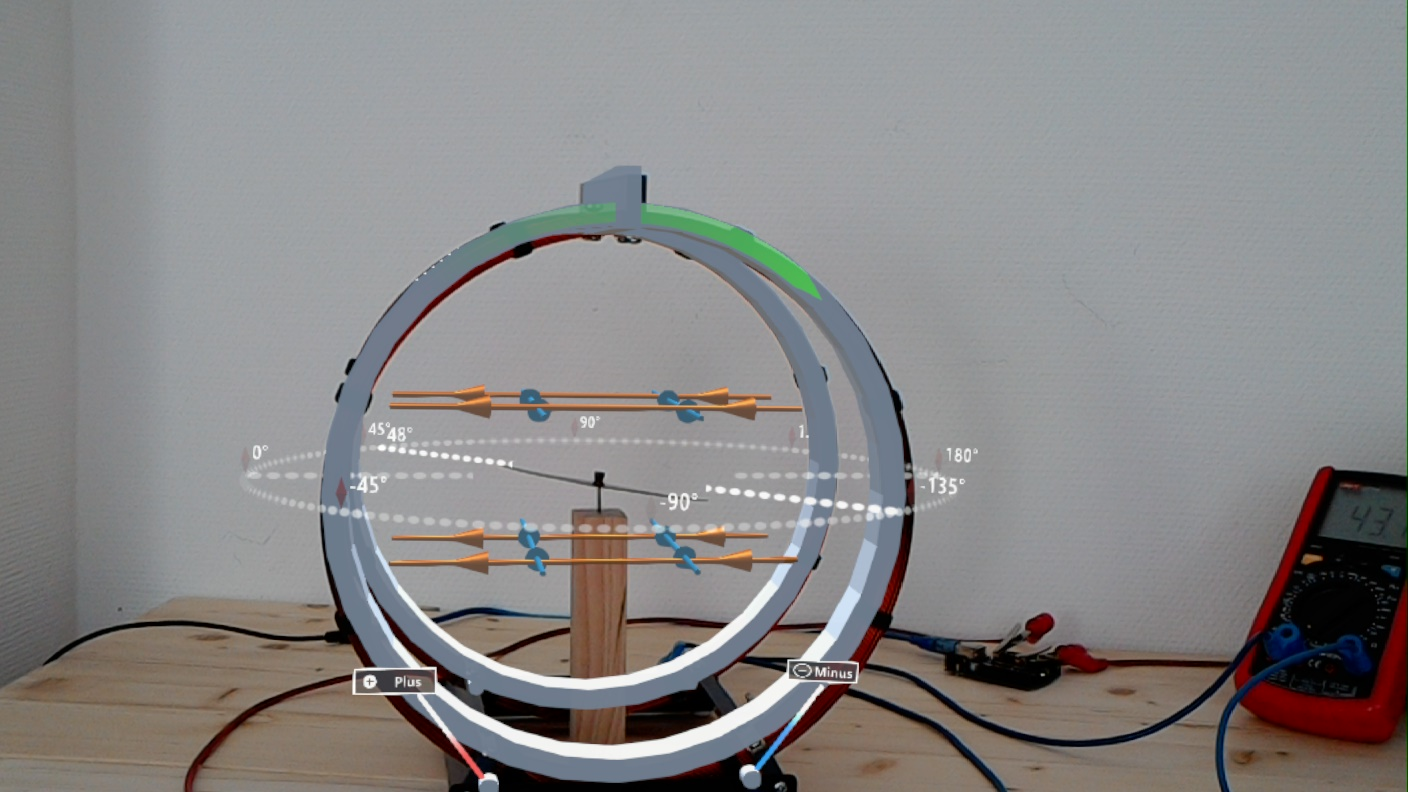
\includegraphics[width=0.48\textwidth]{images/HL/model-overlay.jpg}
	\caption{Überlagerung des virtuellen Modells und der realen Spule. Das virtuelle Modell deckt sich zum großen Teil mit dem realen Objekt. An den Kanten sind jedoch kleine Abweichungen zu erkennen.}
	\label{img:model-overlay}
\end{wrapfigure}
Einen Eindruck von der Güte der Positionierung lässt sich anhand von Abb. \ref{img:model-overlay} gewinnen. Das normalerweise nur in den Tiefenpuffer gerenderte Mesh der virtuellen Spule wird hier durch einen Standard-Shader sichtbar dargestellt. Die reale Spule ist dadurch fast gar nicht zu sehen. Zwar sind Abweichungen zwischen den beiden Objekten aus unterschiedlichen Winkeln unterschiedlich stark sichtbar, das gewählte Foto gibt jedoch einen guten Anhaltspunkt für die tatsächliche Nutzererfahrung wieder.\\

\textit{Interaction Clarity}\\
In Puncto Interaction Clarity kann die Lösung nicht als optimal eingestuft werden. Denn das Kriterium verlangt ausdrücklich, dass eine Anwendung die ihr zu Grunde liegenden Interaktionsmöglichkeiten erklärt, sofern sie über Gewohntes hinausgehen. Das ist bei der Steuerung außerhalb des Menüs nicht der Fall. Die Lösung setzt eine Anleitung durch eine begleitende Person voraus, die den Anwender über die möglichen Aktionen informiert. Die anderen Punkte des Kriteriums werden jedoch erfüllt.\\

\textit{Performance}\\
Die Performance hat maßgeblichen Einfluss auf die Stabilität der Hologramme aber auch der Erweiterbarkeit der Applikation und ist daher von besonderer Bedeutung. Deshalb soll hier der Ressourcenverbrauch etwas ausführlicher beleuchtet werden. Dazu wurde die Anwendung mit Hilfe von Unity's Profiler sowie des Performance Monitores der HoloLens-Weboberfläche analysiert. Der Profiler zeigt unter anderem an, wie lange einzelne Tasks auf Seiten von CPU und GPU benötigen. Der Performance Monitor hingegen zeigt den Ressourcenverbrauch des Gesamtsystems an.\\

Die Anwendung gibt konstant 60 Bilder pro Sekunde aus. Beide genannten Werkzeuge zeigen keine Einbrüche der Framerate. Der Profiler zeigt eine Renderdauer im Bereich von 13 Millieskunden an, wie in Abbildung \ref{img:profiler}. Das liegt noch unter den 16,6 ms zwischen zwei Bildern bei einer Bildwiederholfrequenz 60 Hz. Die Lastverteilung zwischen CPU und GPU variiert dabei, je nach aktiver Darstellung. Die Simulationsdaten und das Tracking verlangen mehr CPU Leistung, während das Rendering der 3D-Objekte die GPU mehr in Anspruch nimmt.\\

TODO...\\
%Einen Überblick über den Ressourcenverbrauch des Gesamtsystems gibt Abbildung \ref{img:performance}. Dabei ist jedoch die Auslastung relativ hoch.

\begin{figure}[h!]
	\centering
	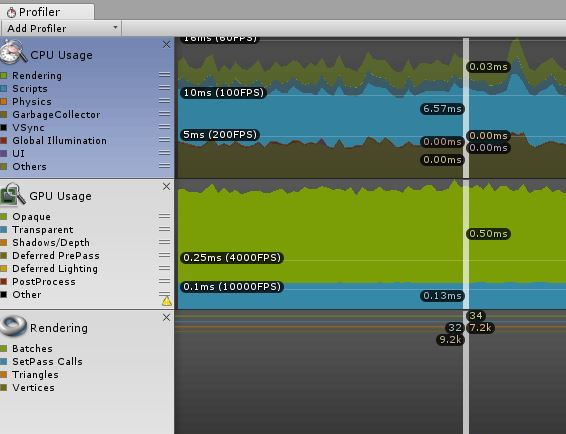
\includegraphics[width=\textwidth]{images/performance/profiler.png}
	\caption{}
	\label{img:profiler}
\end{figure}

Die Kantenglättung wirkt sich deutlich auf den Ressourcenverbrauch der Anwendung aus. Eine Gegenüberstellung der Systemleistungen bei aktiviertem bzw. deaktiviertem Multisampling ist Abbildung \ref{img:msaa-vs-off} zu entnehmen. Unter gleichen Bedingungen steigt die Auslastung der GPU durch 2x MSAA von ca. 40 auf ca. 70 Prozent. Das wirkt sich auch auf den Stromverbrauch aus, der dadurch höher ausfällt, aber noch im akzeptablen Bereich liegt.\\

\begin{figure}[h!]
	\centering
	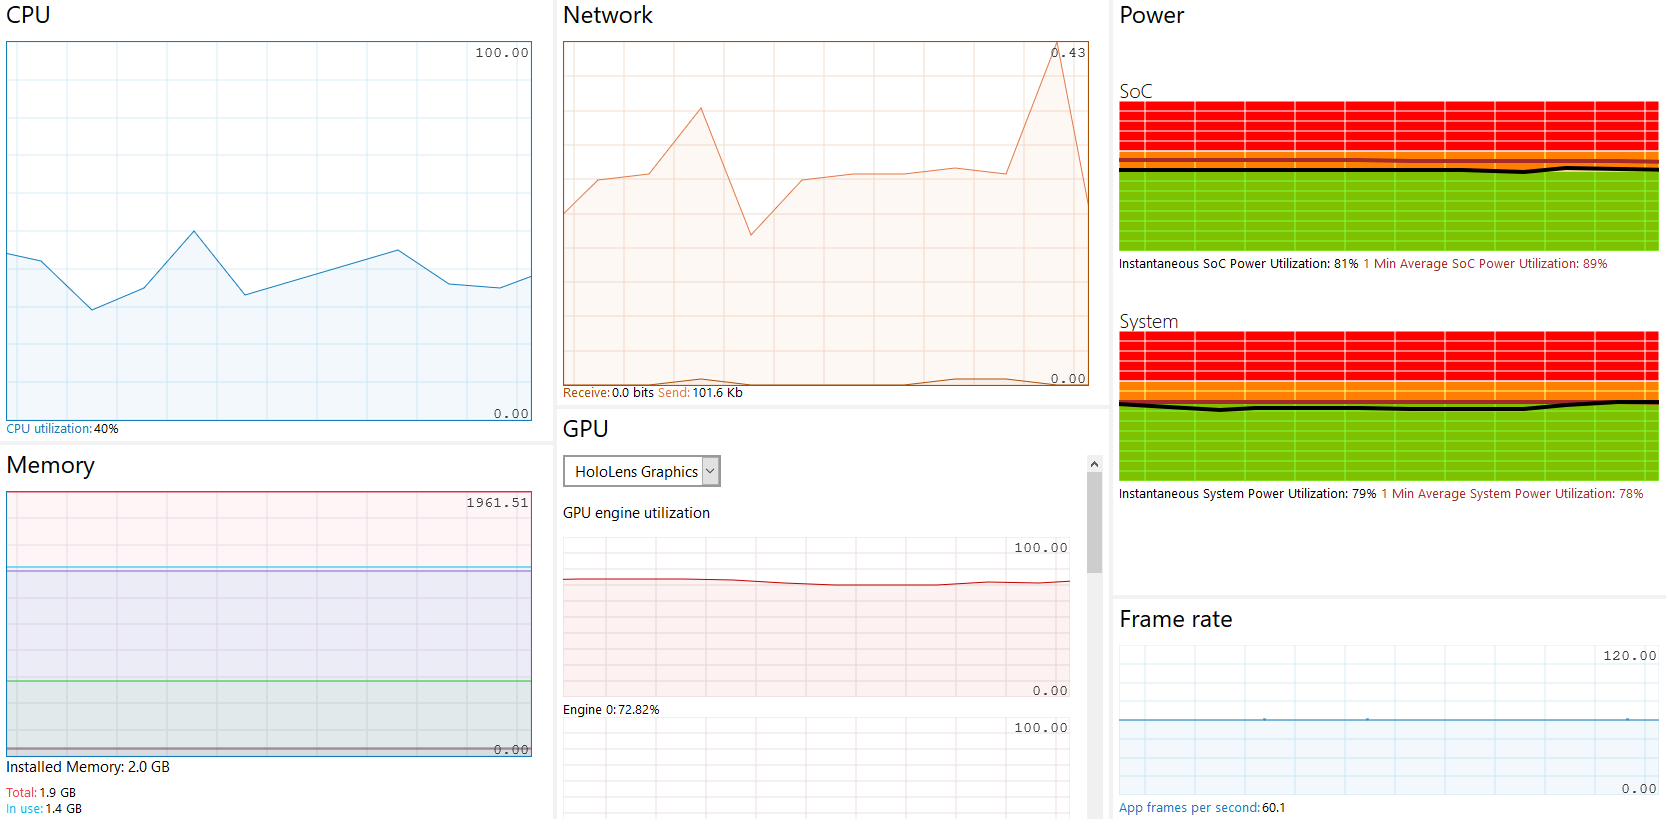
\includegraphics[width=0.45\textwidth]{images/performance/perf_msaa_on.png}
	\hspace{0.05cm}
	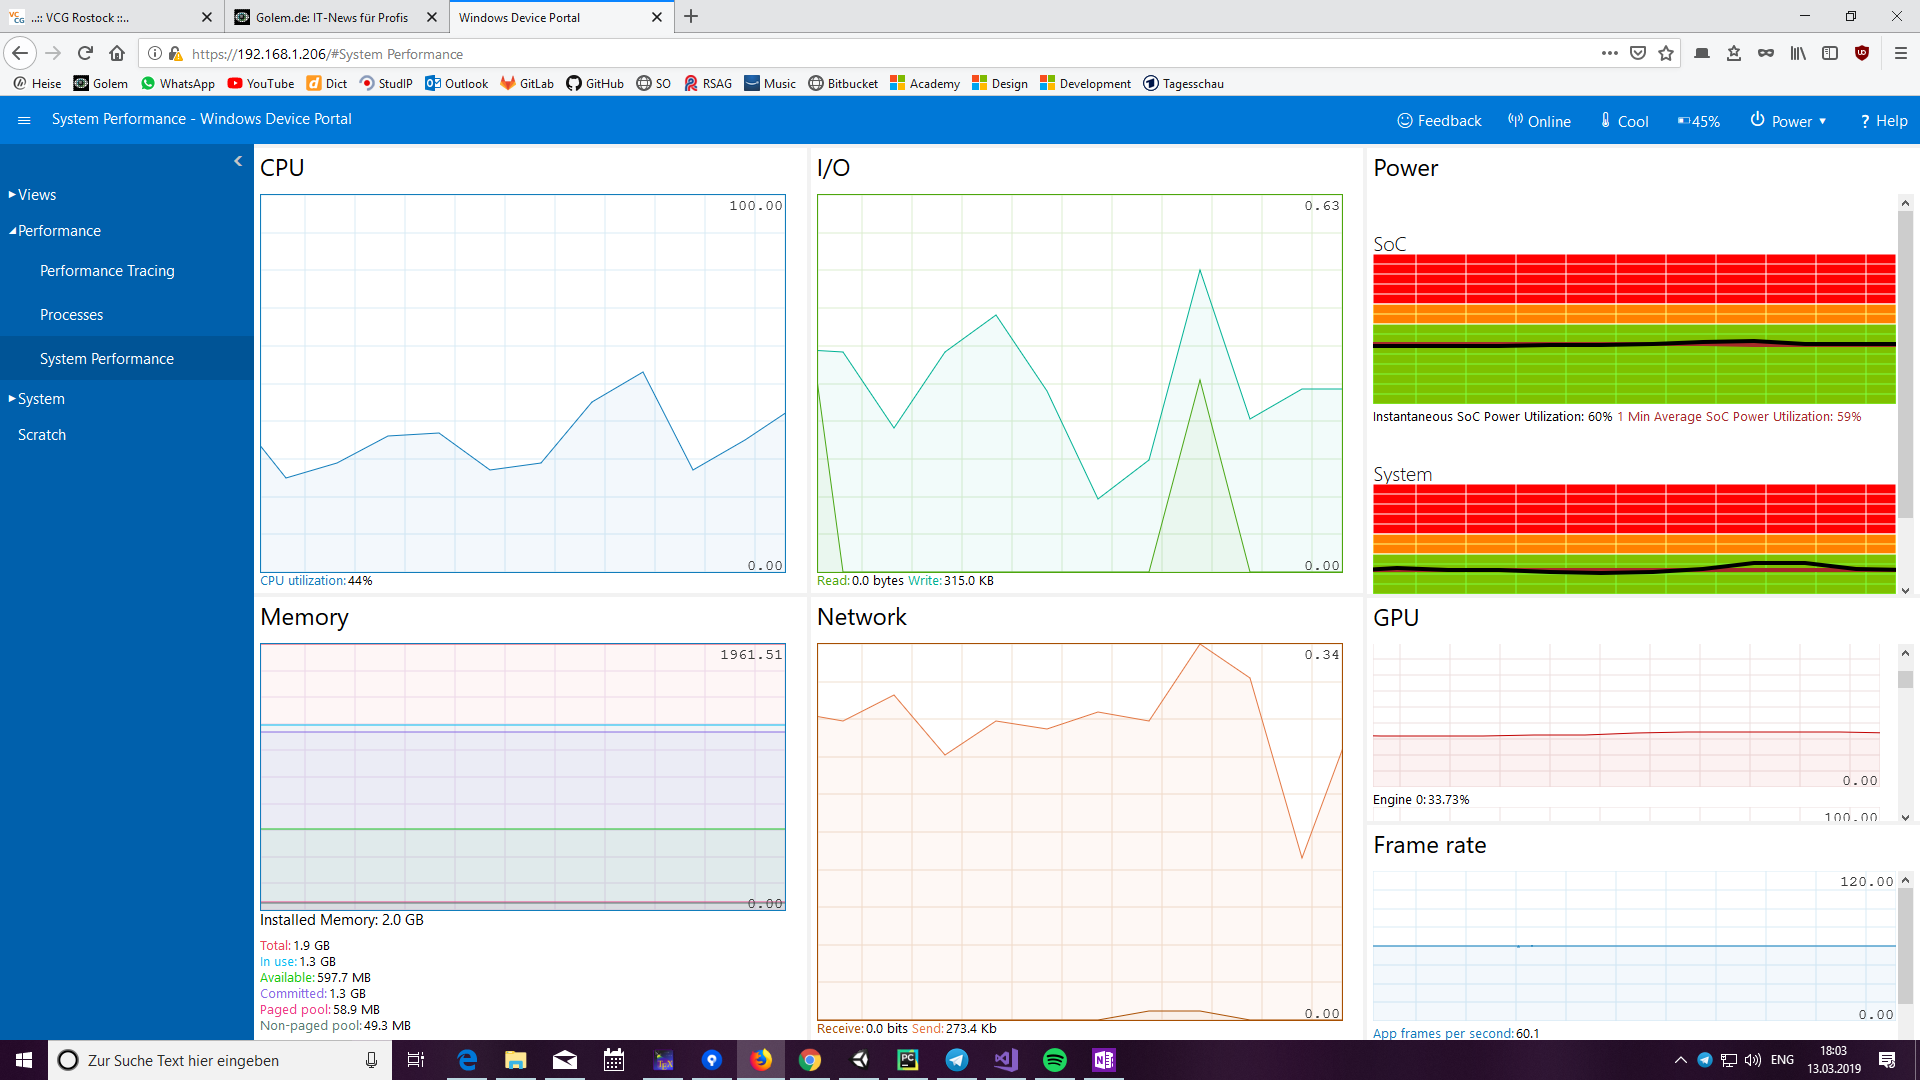
\includegraphics[width=0.45\textwidth]{images/performance/perf_msaa_off.png}
	\caption{Unterschied durch Aktivierung von 2x MSAA. Links ist die Technik aktiviert, rechts nicht, bei sonst gleichen Bedingungen. Die GPU wird ohne MSAA um etwa ein Drittel weniger ausgelastet.}
	\label{img:msaa-vs-off}
\end{figure}


\textit{Testbedingungen}\\
Die Bewertung wurde anhand von Tests unter für die Anwendung günstigen Bedingungen durchgeführt. Der Versuchsaufbau wurde so positioniert, dass die umliegenden Objekte gut für das Tracking der Brille geeignet sind. Außerdem wurde die HoloLens vorher öfter im Testraum verwendet und hatte daher bereits ein gutes Modell des Raums zur Orientierung. Weiterhin wurde die Brille auf den Tester kalibriert und ruckartige oder unnötige Kopfbewegungen vermieden. 

\subsubsection{Feedback}
Zur Bewertung der vorgestellten Lösung wurde die Anwendung außerdem unterschiedlichen Personen vorgestellt und zum Testen überlassen. Dabei handelt es sich um ca. 15 Personen mit unterschiedlichem Grad an Expertise. Das Spektrum umfasst ungefähr zu gleichen Teilen Akademiker, Lehrer und Studenten der Physik. Deren Feedback wurde für diese Arbeit qualitativ festgehalten und zusammengefasst. Die Nutzung der Anwendung beschränkte sich dabei auf den Hauptteil mit den physikalischen Darstellungen.\\

\textit{Inhaltliches Feedback}\\
Die Reaktionen lassen sich weitestgehend als positiv beschreiben. Besonders die Interaktivität und die Darstellung der Simulationsdaten wurden positiv aufgenommen. Bezüglich letzterer wurde gelegentlich nach einer volumetrischen Darstellung gefragt. Die Erfahrung wurde ingesamt meistens als ''Cool'' oder ''Toll'' beschrieben (ohne das nach einer Beschreibung gefragt wurde). Da fast alle Nutzer keine oder fast keine vorangegangenen Erfahrungen mit dem Nutzererlebnis der HoloLens hatten, trägt der ''Wow-Effekt'' einer erstmaligen Nutzung zu den Reaktionen bei.\\

Da viele der Tester Experten waren, gab es kaum Nachfragen zur inhaltlichen Bedeutung der Darstellungen. Typisch waren jedoch Nachfragen zu den Beschränkungen des Sichtfeldes (''Soll das so klein sein?''). Die Rückfrage, ob die Beschränkungen als störend wahrgenommen werden, wurde jedoch meist verneint. Auch die Stabilität wurde als gut wahrgenommen\footnote{Einige Tester wurden ausdrücklich gebeten, ihren Eindruck von der Stabilität zu beschreiben}. Auch zur damit verbundenen Positionierung gab es kein negatives Feedback (z.B. im Falle von nicht korrekt verdeckten Elementen). Negativ fiel hingegen das Kantenflimmern an den Textboxen auf.

\textit{Feedback zur Interaktion und Nutzung}\\
Die Interaktion über den Klicker erwies sich als elementar wichtig. Die Verwendung der Handgeste führte bei unsicheren Nutzern oft zu unerwartetem Verhalten der Anwendung, da die HoloLens Gesten erkannte, die nicht beabsichtigt waren. Weitere Schwierigkeiten betrafen vor allem das Aufsetzen der Brille. Denn wenn diese nicht richtig sitzt, ist das ohnehin schon kleine Sichtfeld nicht vollständig sichtbar. Hier schaffte jedoch eine kurze Erklärung dazu, wie die Brille sitzen sollte, Abhilfe\footnote{Das Feedback zu Sichtfeld, Tragekomfort und Interaktion ist konsistent mit dem Feedback was Microsoft dazu erhalten hat. Alle drei Aspekte wurden deshalb beim Nachfolgemodell massiv verbessert.}.\\

Das Feedback ist nachfolgend noch einmal zusammengefasst.
\vspace{8px}
\begin{center}
	\fbox{
		\parbox{0.9\linewidth}{
			\vspace{4px}
			\textit{Qualitatives Feedback}
			\begin{itemize}[rightmargin=12px, topsep=-12px]
				\setlength{\itemsep}{-1pt}
				\singlespacing
				\item Insgesamt positive Bewertung durch alle Nutzer
				\item Besonders viel positives Feedback zu: 
				\begin{itemize}[topsep=-0.25em]
					\setlength{\itemsep}{-0.25em}
					\item Darstellung der Simulationsdaten 
					\item Interaktivität in Echtzeit
				\end{itemize}
				\item Häufig gewählte Wörter zur Beschreibung der Nutzererfahrung: ''Toll'', ''Cool'' und ''Beeindruckend''
				\item Keine negativen Äußerungen zur Stabilität und Positionierung
				\item Fragen nach einer berechneten Darstellung für 3D			
				\item Klicker wurde den Handgesten stets vorgezogen				
				\item Anmerkungen zu hohem Aufwand und Praktikabilität
				\item Viele wollten Fotos der Anwendung haben
				\item Kaum Feedback von Lernenden, fast allen Nutzern waren die physikalischen Zusammenhänge bereits zu großen Teilen oder vollständig bekannt
			\end{itemize}
			\vspace{18px}
	}}\\
\end{center}
\vspace{6px}

\subsection{Diskussion}
TODO...\\

KRITISCH MIT DER EIGENEN ARBEIT AUSEINANDERSETZTEN!!\\

Kantenflimmern unerwartetes Problem. Kantenglättung zu teuer und nicht ausreichend. Kanten anders glätten. Keine weißen Linien und Umrandungen verwenden.\\

Einige Probleme konnten bereits im Design abgemildert oder umgangen werden. Das gilt z.B. für die Aspekte Komfortzone und FOV-Grenzen. Durch die platzsparende Anordnung der Elemente werden die Hologramme seltener abgeschnitten. Außerdem sind häufige Kopfbewegungen und Hinweise auf Elemente außerhalb des FOV so nicht notwendig. Und die Berücksichtigung einer geeigneten Distanz von Beginn an vermeidet bzw. verringert Probleme mit zu dicht positionierten Objekten.\\

Hier wurde z.B. bei der Festsetzung von Anzahl und Größe von Objekten auf die Einschränkungen der HoloLens Rücksicht genommen. Viele Probleme werden auch durch die Nutzung von vorgefertigten Objekten und Verhaltensweisen vermieden. Hier sind z.B. der Progress Indikator, Standard-Button und Standard-Shader zu nennen.\\

Nicht für alles muss eine softwareseitige Lösung her, siehe z.B. Begrenzung der Darst. und aufgehellte Magnetnadel.\\

Frage: Wie HoloLens einsetzen?

\begin{itemize}
	\item Über 3D-Darstellungen Felder im Raum anzeigen, profitiert von stereoskopischer Wahrnehmung und See-Through-Displays
	\item Empfohlene Verhaltensweisen durch Nutzung von vorgefertigten Elementen einbinden
	\item Interaktion einfach halten, z.B. durch Klicker
	\item Zusammenspiel von realen und virtuellen Objekten nutzen, nicht für alles muss eine softwareseitige Lösung geschaffen werden
	\item Virtuelle Objekte an Versuchsaufbau verankern, dadurch verliert Nutzer sie nicht
	\item Tracking der HoloLens nutzen, um Objekte zu positionieren, anstelle eines dauerhaft sichtbaren Markers, Stabilität ausreichend, dabei aber mögliche Störfaktoren beachten...
	\item ... Stabilität bei diesem Ansatz wichtig, daher Performance sehr wichtig, unbedingt beachten und Optimierungen vornehmen
	\item World Anchor kann für grobe Positionierung genutzt werden, um Setup-Zeit zu verringern
	\item Anwendung ist hochgradig zugeschnitten auf die konkreten Eigenschaften des Experimentes
	\item Einsatz per Streaming denkbar, dann jedoch weitere perf. Opt. notwendig oder Deaktivieren von MSAA
	\item Anpassbarkeit
\end{itemize}

Wie die HoloLens weiter im Kontext des gewählten Versuches verwendet werden könnte.

\subsubsection{Erweiterbarkeit}
Ein im Rahmen der Fragestellung wichtiger Aspekt besteht darin, wie die vorgestellte Lösung um weitere Inhalte erweitert werden könnte. Dies ist in mehreren Bereichen denkbar und soll im Folgenden diskutiert werden.\\

Eine zuvor bereits angedeutete Erweiterung bestünde darin, mit Erklärungen durch die Anwendung und Durchführung des Experimentes zu führen. Dabei könnten die Darstellungsmodelle und physikalischen Zusammenhänge erläutert, aber auch Hinweise zur Nutzung gegeben werden. Auf diese Weise ließe sich beispielsweise kommunizieren, wie die Darstellungen zu interpretieren sind oder welche Interaktionsmöglichkeiten zur Verfügung stehen. Eine Umsetzung wäre beispielsweise mittels Animationen und eingesprochenen Texten denkbar. Im Zuge einer solchen Erweiterung ließe sich die Anwendung auch gezielt auf ein konkretes Einsatzszenario wie z.B. den Einsatz in einer Unterrichtsstunde auslegen.\\

Die in der Simulation berechneten Feldlinien geben das Feld in einem 2D-Schnitt wieder. Diese Darstellung ließe sich zu einer 3D-Darstellung erweitern. Dafür müssten auf Seiten der HoloLens zunächst keine weiteren Anpassungen vorgenommen werden, sofern die Daten in einer Datei im entsprechenden Format bereitgestellt werden. Allerdings sind die knappen Ressourcen zu berücksichtigen. Eine größere Anzahl an Feldlinien könnte zu einem Einbruch der Framerate führen. Eine mögliche Lösung bestünde darin, die Anzahl und bzw. oder Granularität der Feldlinien anzupassen. Alternativ ließen sich auch Qualitätseinstellungen (z.B. MSAA, Auflösung) auf der HoloLens verändern, um den Ressourcenverbrauch einzuschränken.\\

Außerdem wäre eine Variation der physikalischen Parameter umsetzbar. Dazu zählen unter anderem Radius, Windungszahl, elektrischer Widerstand und Materialeigenschaften. Die physikalischen Berechnungen sind parametrisiert und ließen sich zur Laufzeit anpassen. Dadurch könnten auch die Zusammenhänge zwischen diesen Parametern und dem entstehenden Magnetfeld beleuchtet werden.\\

Grundsätzlich sind auch Erweiterungen um weitere Lerninhalte denkbar, die mit dem Versuch zusammenhängen. Beispielsweise wäre eine explizite Erklärung des Zusammenhangs zwischen Stromrichtung, Flussrichtung der Elektronen und Richtung des entstehenden Magnetfeldes möglich. Dies ließe sich auch Erweitern auf eine Aufbereitung des Biot-Savart-Gesetzes, dass allgemein die Magnetfelder bewegter Ladungen im Raum beschreibt und auf dem auch die Feldgleichungen der Helmholtz-Spule beruhen. Allerdings ist die Architektur der Applikation nicht explizit auf weitere, eigenständige Szenarien ausgelegt.\\

\subsubsection{Übertragbarkeit}
Ansatz übertragen auf andere Versuche:

Neben dem vorgestellten Experiment sind mit einer Helmholtz-Spule noch weitere Versuche möglich. Ein typisches Beispiel ist die Ablenkung eines Elektronenstrahls, der durch ein Gas sichtbar gemacht wird. Die Elektronen werden im Inneren der Spule durch das Magnetfeld entsprechend dessen Stärke abgelenkt. In dem Versuch ist letztere so einzustellen, dass die Elektronen auf eine Kreisbahn gezwungen werden.\\

Durch die vielen Gemeinsamkeiten mit dem in dieser Arbeit behandelten Versuch liegt eine Übertragung der Lösung auf diesen Anwendungsfall nahe. Das Magnetfeld, die Stromrichtung und die Echtzeitdaten könnten hier ebenfalls in den Versuch integriert werden. Dabei wären jedoch ggf. andere Anforderungen durch den geänderten Versuchsaufbau zu berücksichtigen.\\

Ebenfalls denkbar wäre eine Übertragung auf ähnliche Versuche. Hier käme beispielsweise die Ablenkung eines Elektronenstrahls durch Plattenkondensatoren in Frage. Diese erzeugen ein elektrisches Feld, durch das Elektronen abgelenkt werden\footnote{Eine interaktive Webanwendung zu diesem Versuch findet sich hier: \url{https://www.didaktik.physik.uni-muenchen.de/elektronenbahnen/e-feld/hypothesen/experiment.php}}. Die Felddarstellungen können auch für elektrische Felder genutzt werden und auch die Labels für Plus und Minus ließen sich übernehmen.\\

Grundsätzlich ist die Übertragbarkeit jedoch eingeschränkt, da die Lösung stark auf den Anwendungsfall und dessen Eigenschaften zugeschnitten ist. Bei einem anderen Versuch lassen sich Darstellungen ggf. nicht auf die gleiche Weise einbetten. Wenn z.B. der Nutzer ständig mit realen Objekten direkt interagieren muss, an denen die virtuellen Objekte verankert sind, wird die Empfohlene Distanz zu den Darstellungen dauerhaft unterschritten. Außerdem schaffen bewegliche Objekte, deren Position verfolgt werden muss, zusätzliche Probleme. Ein fortlaufendes Tracking durch die HoloLens über optische Merkmale nimmt massiv Ressourcen in Anspruch und führt dazu, dass keine Aufnahmen der Anwendung von der HoloLens selbst gemacht werden können.\\

Die Probleme können durchaus sehr individuell sein. Im Falle des zuvor genannten Versuches mit der Ablenkung des Elektronenstrahls könnte beispielsweise ein Problem mit dem Tracking auftreten. Wenn nämlich das Licht ausgeschaltet werden muss, damit der Elektronenstrahl zu erkennen ist, verliert die HoloLens ggf. aufgrund der mangelnden optischen Merkmale die Orientierung. Experimente mit zu hellen Elementen sind jedoch auch problematisch, da dann die Hologramme schlechter sichtbar wären. Aber auch andere Quellen von Infrarotlicht sowie stark reflektierende oder transparente Materialien würden das Tracking stören. Nicht zuletzt spielt auch Sicherheitsausrüstung eine Rolle. Bei einem Experiment mit einem Laser ist ggf. eine Schutzbrille notwendig, die den Einsatz der HoloLens möglicherweise ausschließt.\\

Für ein konkretes Experiment ist folglich individuell zu prüfen, in wie fern die technischen Voraussetzungen der eines Einsatzes der HoloLens gegeben sind.
	
	
	
	
	
	
	
	
	
	
	